\documentclass{article}

\usepackage[letterpaper, portrait, margin=1.5in]{geometry}

\usepackage{fancyhdr}
\usepackage{ragged2e}
\usepackage{graphicx}
\usepackage{caption}
\usepackage{amsmath}
\usepackage{rotating}

\usepackage{listings}
\usepackage{color}

\definecolor{dkgreen}{rgb}{0,0.6,0}
\definecolor{gray}{rgb}{0.5,0.5,0.5}
\definecolor{mauve}{rgb}{0.58,0,0.82}

\lstset{frame=tb,
  language=Java,
  aboveskip=3mm,
  belowskip=3mm,
  showstringspaces=false,
  columns=flexible,
  basicstyle={\small\ttfamily},
  numbers=none,
  numberstyle=\tiny\color{gray},
  keywordstyle=\color{blue},
  commentstyle=\color{dkgreen},
  stringstyle=\color{mauve},
  breaklines=true,
  breakatwhitespace=true,
  tabsize=4
}

\setcounter{secnumdepth}{1}

\usepackage{chngcntr}
\counterwithin{figure}{section}

\renewcommand*{\thepage}{C\arabic{page}}

\pagestyle{fancy}
\lhead{ACME Robotics}
\chead{\#8367}
\rhead{\ifcontents Contents \else Week \thesection \fi}

\newif\ifcontents
\contentstrue

\makeatletter
\renewcommand{\@seccntformat}[1]{}
\makeatother
\begin{document}

\subsection{Write Mecanum Drive Code}
As Emma will potentially be the only software person on ACME next year, she needs to learn as much as she can about the team's current software to prepare for next year. Emma has not done a lot of robot code in the past, but she was ready to give it a go. Along with that, Emma is also going to learn how Road Runner, the motion planning libraries the team developed, works. The team has a still assembled mecanum drive base from the Relic Recovery robot. This base is perfect for what Emma is trying to do. She decided that instead of jumping straight into figuring out motion planning, she should probably write a mecanum drive program to begin. Emma had written tank drive code before, but never mecanum. This seemed like an apt challenge for the time being. \\

Emma did quite a bit of research on mecanum drive code before settling down to write hers. She found that there are a lot of different ways to write mecanum drive, some more complicated than others. She found an equation for mecanum drive, as seen in Figure \ref{fig:equation} that she thought she could work off of. Basically, the equation takes the desired robot speed, multiplies it times the sine/cosine of the desired robot angle minus pi over 4, and finally adds/subtracts that to the desired speed when the robot changes direction in order to get the actual speed of the robot. \\

\begin{figure}
    \centering
    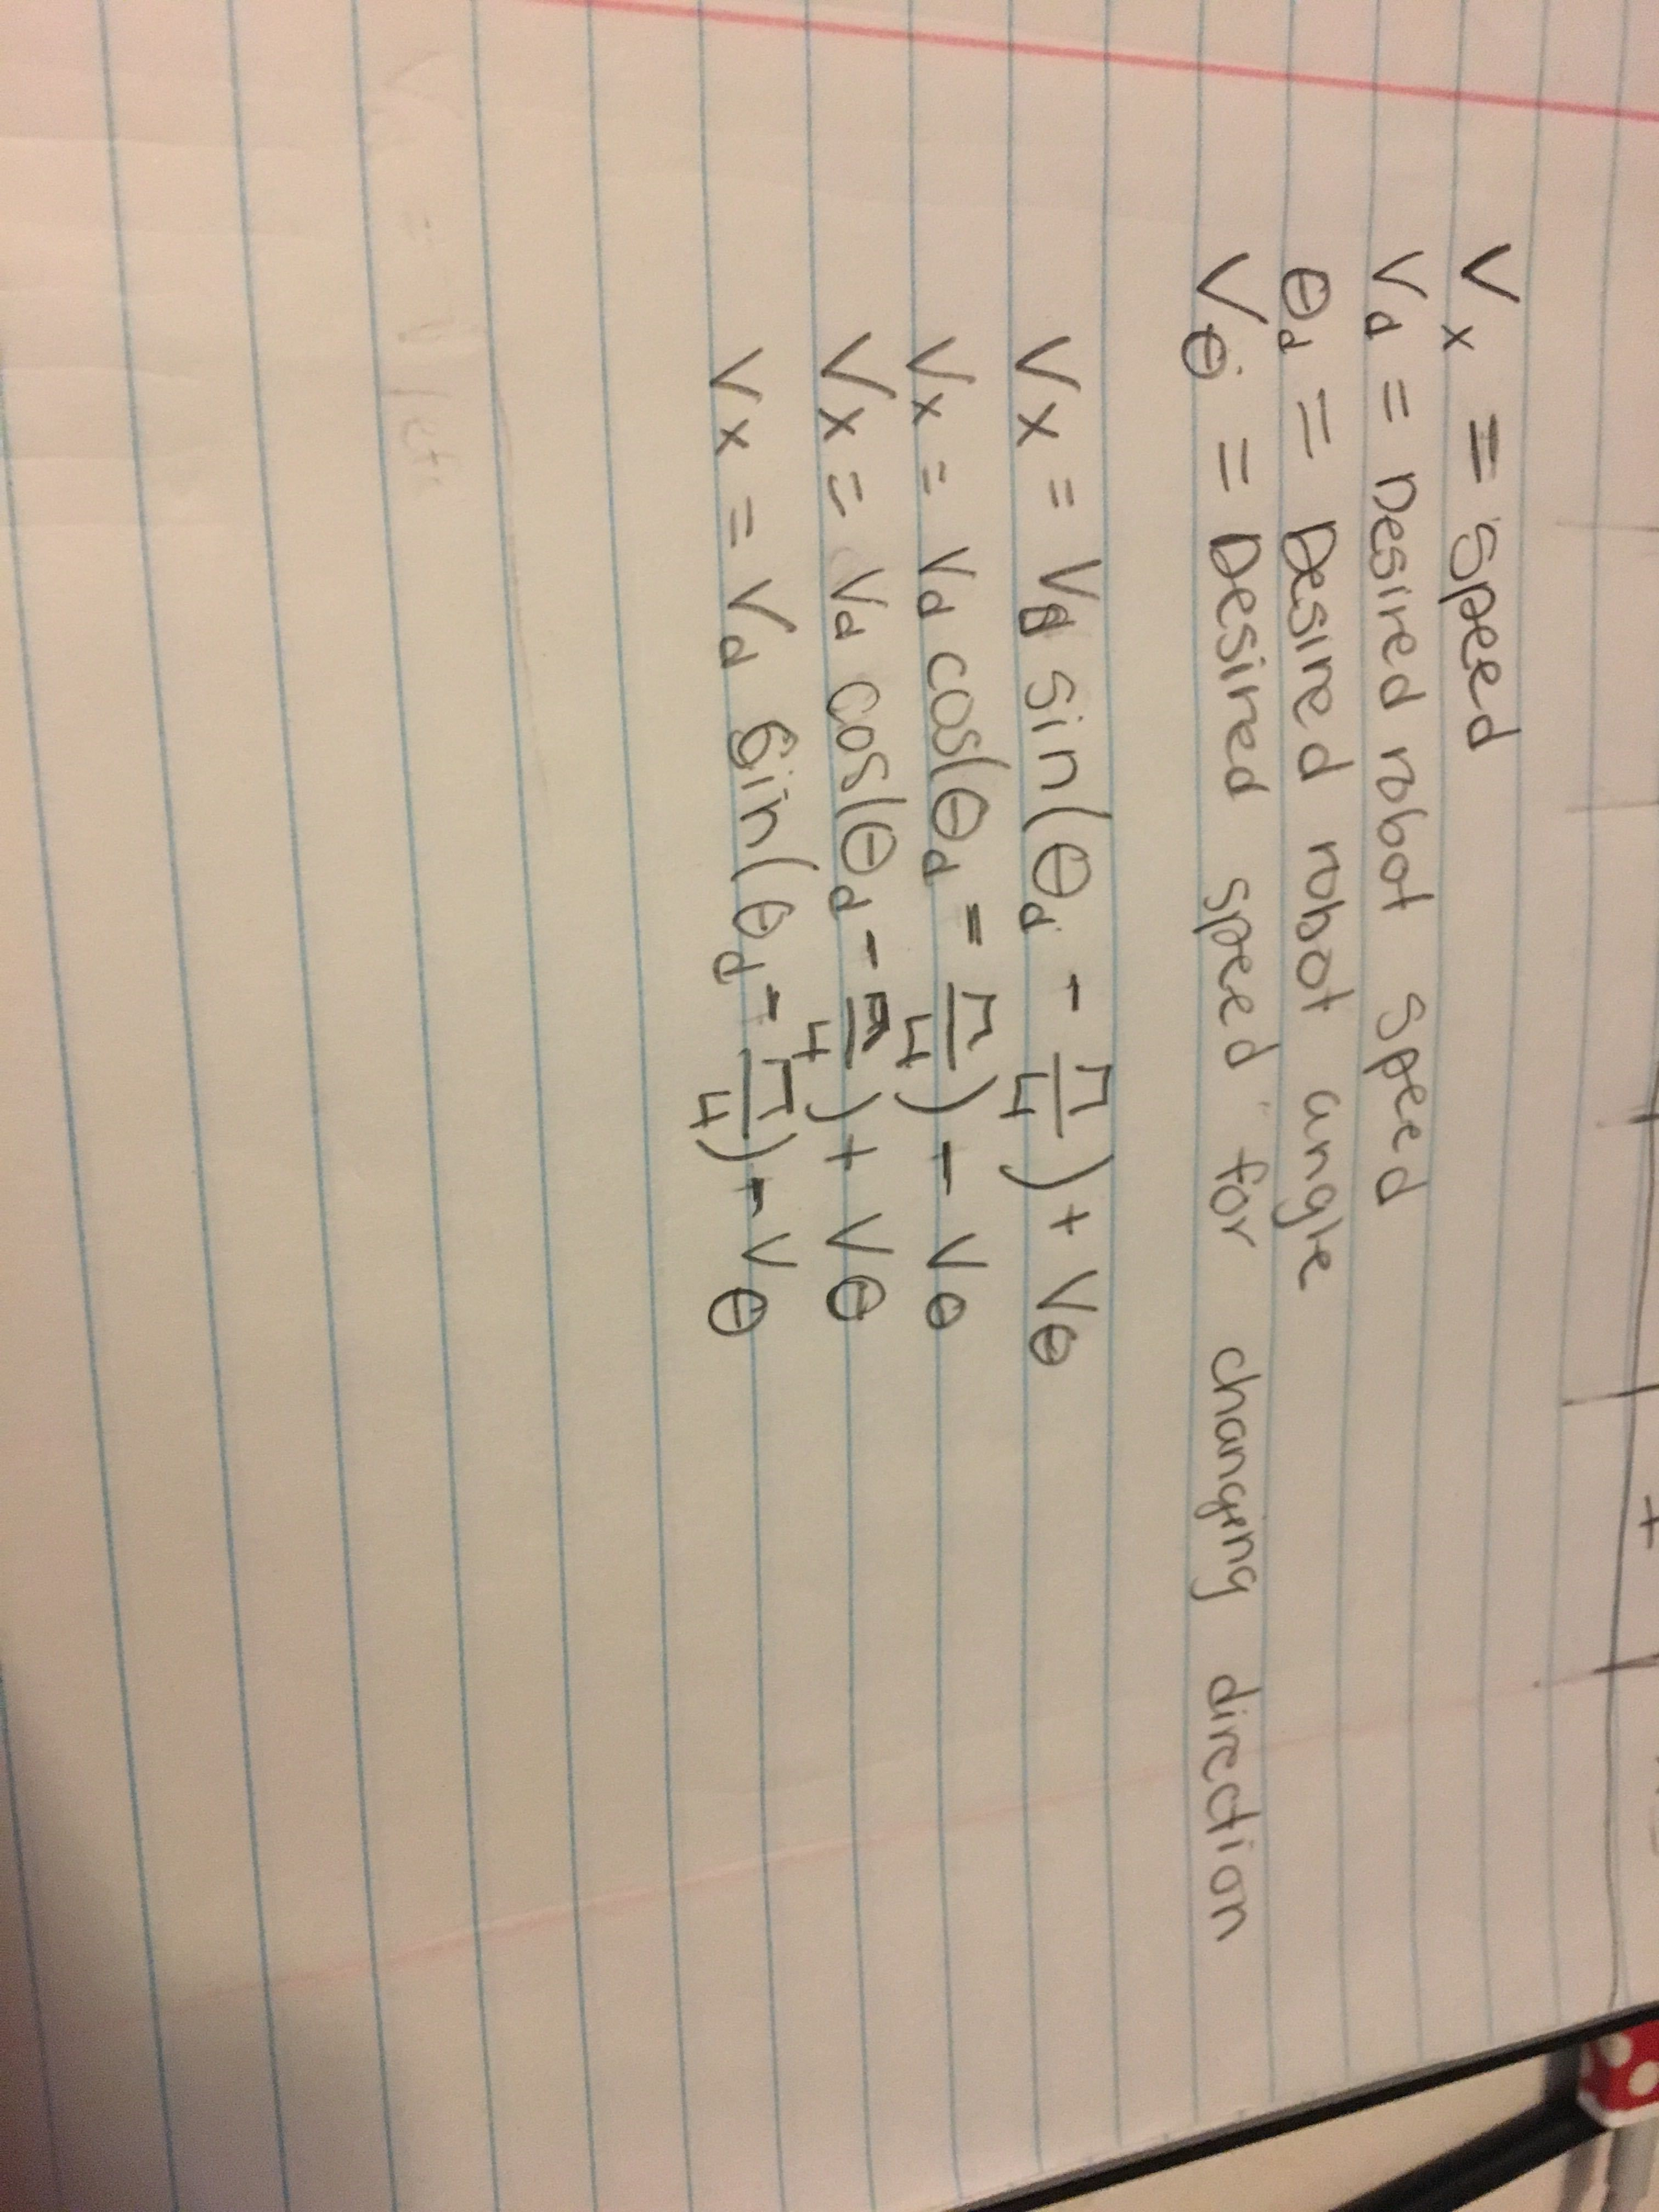
\includegraphics[width= 0.5 \textwidth, angle=90 ] {29_03-18/images/equation.JPG}
    \caption{Equation Used for Mecanum Drive Code}
    \label{fig:equation}
\end{figure}

To begin to put this into code, Emma wrote a TeleOp program. She found the hypotenuse of the left joystick's x and y position. Then she found the arc tangent of the left joystick's x and y position and subtracted pi over 4 from that. Finally, she made a double called ''turn" which took the value of the right joystick's x position (which is the control used to turn the robot). Using all of this information, she filled in the equation as see in Figure \ref{fig:equation}. Below, there is the code that controls the front left wheel and the front right wheel of the robot (the code for the back left and right wheels is the same). \\

\newpage
\begin{lstlisting}[language=Java]
double speed = Math.hypot(gamepad1.left_stick_x, gamepad1.left_stick_y);
double angle = Math.atan2(gamepad1.left_stick_y, gamepad1.left_stick_x);
double turn = gamepad1.right_stick_x;

final double lfPower = speed * Math.sin(angle) + turn;
final double rfPower = speed * Math.cos(angle) - turn;

leftFront.setPower(lfPower);
rightFront.setPower(rfPower);
\end{lstlisting}

At the final meeting of this week, Emma wanted to test her code on the mecanum drive base. After doing some cable management and setting up the configuration, she ran the program. Emma ended reversing two of the motors in order to get them all going in the right direction when she pressed forward, but other than that the code worked perfectly! \\


\end{document}